\documentclass[a4paper,12pt]{article}
\usepackage{mathtools,amsfonts,amssymb,amsmath, bm,commath,multicol}
\usepackage{algorithmicx, tkz-graph, algorithm, fancyhdr, pgfplots}
\usepackage{fancyvrb}

\usepackage[noend]{algpseudocode}

\pagestyle{fancy}
\fancyhf{}
\rhead{27/2/2017 ::: Nandan Rao}
\lhead{Machine Learning ::: Problemset 3}
\rfoot{\thepage}


\DefineVerbatimEnvironment{juliaout}{Verbatim}{}
\DefineVerbatimEnvironment{juliacode}{Verbatim}{fontshape=sl, fontsize=\tiny}
\DefineVerbatimEnvironment{juliaterm}{Verbatim}{}


\begin{document}

\section*{9}

\subsubsection*{Rademacher Average of Unions}
The rademacher average of the union of two sets is the expectation of the supremum of a union of two sets:
$$
R_n(A \cup B) = \mathbb{E} \ \sup_{c \in A \cup B} \ \frac{1}{n} | \sum \sigma_i c_i |
$$
%
The supremum of a union of two sets A and B must, naturally, be equal to the supremum of either set A or set B:
$$
\sup_{c \in A \cup B} f(c) = \sup_{a \in A} f(a) \ \ or \ \  \sup_{b \in B} f(b)
$$
Because rademacher averages are, due to the absolute-value sign, non-negative numbers:
$$
\mathbb{E} \ \sup_{a \in A } \ \frac{1}{n} | \sum \sigma_i a_i | \geq 0
$$
Which leads to the following result:
\begin{align*}
R_n(A \cup B) &\leq \mathbb{E} \ \sup_{c \in A \cup B} f(c) + \text{non-negative number} \\
R_n(A \cup B) &\leq \mathbb{E} \ \sup_{a \in A } \ \frac{1}{n} | \sum \sigma_i a_i | + \mathbb{E} \ \sup_{b \in B} \ \frac{1}{n} | \sum \sigma_i b_i | \\
R_n(A \cup B) &\leq R_n(A) + R_n(B)
\end{align*}

\subsubsection*{Rademacher Average Multiplied By a Constant}
This is shown by the fact that we can move a constant outside of a sum, we can move a constant outside of a supremum (all possibilities are multiplied by the constant, so the constant does not help us compare), and we can move a constant ourside of an expectation:
\begin{align*}
R_n(c \cdot A) &= \mathbb{E} \ \sup_{a \in A} \ \frac{1}{n} | \sum c \sigma_i a_i | \\
R_n(c \cdot A) &= \mathbb{E} \ \sup_{a \in A} \ \frac{1}{n} | \ c \ | \cdot \ | \sum \sigma_i a_i | \\
R_n(c \cdot A) &= \mathbb{E} \ | \ c \ | \sup_{a \in A} \ \frac{1}{n} \cdot \ | \sum \sigma_i a_i | \\
R_n(c \cdot A) &= | \ c \ | \ \mathbb{E} \  \sup_{a \in A} \ \frac{1}{n} \cdot \ | \sum \sigma_i a_i | \\
R_n(c \cdot A) &= | \ c \ | R_n(A)
\end{align*}

\subsubsection*{Rademacher Average of Direct Sums}

\begin{align*}
R_n(A) + R_n(B) &\geq R_n(A \oplus B) \\
R_n(A) + R_n(B) &\geq \mathbb{E} \ \sup_{a \in A, b \in B } \ \frac{1}{n} | \sum \sigma_i (a_i + b_i) | \\
R_n(A) + R_n(B) &\geq \mathbb{E} \ \sup_{a \in A, b \in B } \ \frac{1}{n} | \sum \sigma_i a_i + \sigma_i b_i | \\
R_n(A) + R_n(B) &\geq \mathbb{E} \ \sup_{a \in A, b \in B } \ \frac{1}{n} | \sum \sigma_i a_i + \sum \sigma_i b_i |
\end{align*}
In the largest case, the supreme of the two sums will be equal to the two sums of the supremums, else they might be lesser. This is essentially the triangle inequality:
$$
\mathbb{E} \ \sup_{a \in A } \ \frac{1}{n} | \sum \sigma_i a_i | + \mathbb{E} \ \sup_{b \in B} \ \frac{1}{n} | \sum \sigma_i b_i | &\geq \mathbb{E} \ \sup_{a \in A, b \in B } \ \frac{1}{n} | \sum \sigma_i a_i + \sum \sigma_i b_i | \\
$$


\section*{10}

\subsubsection*{VC Dimension of a Circle}

I claim that the VC dimension of a circle is 3. To prove this, we need to prove it is impossible for a circle shatter any 4 points in $\mathbb{R}^2$. \\
\\
Consider any 4 points ${a,b,x,y} \in \mathbb{R}^2$. Pick the two points who lie furthest from each other and call them a and b, respectively, and the distance between them d. The smallest circle that contains both a and b can be described as follows:
$$
C_{a,b \in C} = \big\{ x \in \mathbb{R}^2 : || x - c \leq \frac{d}{2}|| \big\}
$$
Where the center-point of the circle, c, is half-way between a and b:
$$
a - c = b - c = \frac{d}{2}
$$
All other points must lie within distance d of both a and b (otherwise a and b would not be the furthest points).
$$
x - a, x - b, y - a, y - b \leq d
$$
Again, because a and b are the furthest points, we know that:
$$
x - y \leq d
$$
The quadralateral formed by ${a,b,x,y}$ has, therefore, a maximum diagonal dimension of d, the distance between a and b. Any quadralateral with maximum diagonal distance d, however, is fully contained within a circle whose center-point is the center of that maximum diagonal distance and radius is $\frac{d}{2}$. Therefore, even the smallest possible circle containing the two furthest points cannot possibly exclude the other two, and therefore cannot fully shatter the space. \\
\\
Proving that a circle can shatter 3 points is trivial, we simply need to consider an equilateral triangle, with edges of distance h, and consider a circle with radius $\frac{h}{2}$. Placing this circle on the (3) centers of the edges and on the (3) vertices will create all 6 partial sets of the three points. The final set is any circle larger than the equilateral triangle, the empty set is trivial, and you have all $2^3$ combinations. The VC dimension of a circle must, therefore, be 3.

\subsubsection*{VC Dimension of a Circle with Radius 1}
The VC dimension is, by construction, a worst-case scenario measurement. Restricting the size of the circle, without restricting the space of the data (by, for example, setting a minimum distance of the points to each other point), will lead to the exact same VC dimension, as we can simply scale the points in the previous examples, and obtain the same dimension.

\section*{11}

\subsubsection*{Shatter Coefficient of a Half-Plan}
$$
A_0 = \big\{ H_{a,b,c} : a,b,c \in \mathbb{R}^2 \big\}
$$
%
Let us first agree that the worst-case scenario for a half-plane classifier (a linear classifier) is when all the points lie on the edge of their convex hull. Let us consider N such points, $p_1, p_2,...,p_N$. Consider the half-plane that runs tangent to point $p_1$ and classifies every point it runs through and to the right of the line as 1, and everything else as 0. In its current position, this classifies only itself as 1. Now rotate this half-plane, using as a fulcrum $p_1$, to go in-between all the other points on the hull (N - 2 other positions, between each of the N - 1). Repeat this process until $p_N$. This leaves us with:
$$
N(1 + N - 2)
$$
%
Now we add the full set and the empty set, and we find our shatter coefficient:
$$
N(N - 1) + 2
$$
\subsubsection*{Shatter Coefficient of Origin-Fixed Half-Plan}
$$
A_0 = \big\{ H_{a,b,0} : a,b \in \mathbb{R}^2 \big\}
$$
%
Considering a similar arrangement as before, with all points on the edge of their convex hull, and instead of placing our origin on one of the points, we will place it on an edge. Rotate it through all the points as before, giving you $1 + N - 2$ sets again. Now multiply the sets by 2 because you can flip the sign (we didn't do this before because this was accounted for when we moved our fulcrum points). This gives us $2(N - 1)$. Now add the empty and full sets (this is why we placed it on an edge, not on a point!). This leaves us with:
$$
2N
$$

\section*{12}
The plot of what happens holding the dimension fixed and increasing the sample size is fairly intuitive. Both increasingly get better, as their approximate bounding box approaches the truthful one of the data generating process. What is interesting is their different minimum level of asymptotic error. The cube classifier will always perform at least as well as the rectangle, as it is replicating our data-generating process, and the rectangle classifier can also be considered to be overfitting the training data. It has a higher VC dimension!! We see this play a bigger role in high dimensions, where the cube, with every increase in dimension, approaches the true numbers, while the rectangle classifier simply increases its ability to overfit the training data. The cube has a constant error rate accross dimensions, which can be explained by the fact that the probability of the minimum/maximum coordinates being mismatched with the true ones is the same probability that causes damage in the testing, but helps it in the training, so the interaction between the two stays constant with growing dimensionality.




\subsubsection*{Training Size, test size 500, dimensions 10, mean of 50 trials}
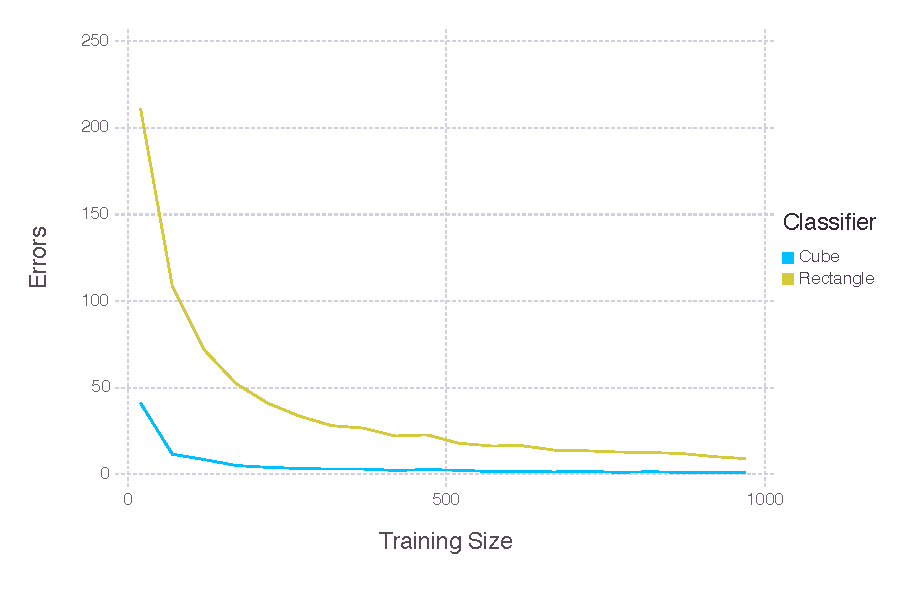
\includegraphics[width=\linewidth]{figures/problemset3_2_1.pdf}



\subsubsection*{Dimensions, test size 500, training size 100, mean of 50 trials}
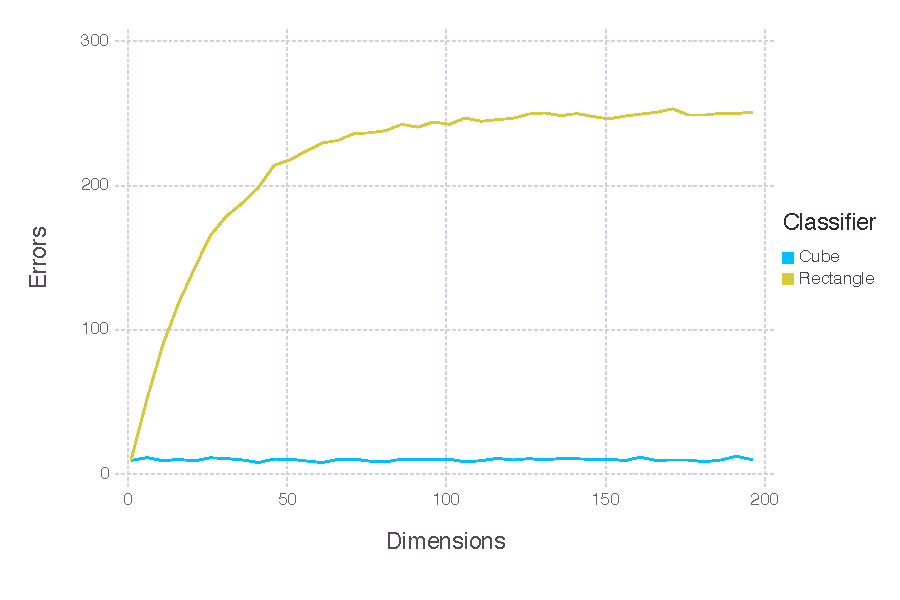
\includegraphics[width=\linewidth]{figures/problemset3_3_1.pdf}



\section*{Code}
\begin{juliacode}
using Base.Test
using DataFrames
using Gadfly

function generate_X(N, d = 3)
    rand(N, d)*2*2^(1/d) - 2^(1/d)
end

@test maximum(generate_X(100, 3)) <= 2^(1/3)
@test maximum(generate_X(100, 6)) <= 2^(1/6)
@test size(generate_X(100, 5)) == (100, 5)

function should_be_one(X::AbstractArray{Float64}, min = -1.0, max = 1.0)
    all([x <= max && x >= min for x in X])
end

function should_be_one(x::Float64, min = -1.0, max = 1.0)
    x <= max && x >= min
end

@test should_be_one(1.5) == false
@test should_be_one([-.5, .5]) == true
@test should_be_one([-.5, 1.5]) == false

function label_X(X, fn)
    [fn(X[i,:]) ? 1 : 0 for i in 1:size(X)[1]]
end

function get_edges(X)
    [(minimum(X[:,d]), maximum(X[:,d])) for d in 1:size(X)[2]]
end

function get_ones(X, Y)
    ones = [X[i,:]' for i in 1:length(Y) if Y[i] == 1]
    length(ones) > 0 ? reduce(vcat, ones) : ones
end

@test get_ones([1,2,3], [0,0,0]) == []
@test get_ones([1 2 3; 4 5 6], [1,1]) == [1 2 3; 4 5 6]

function get_corners(edges)
    m = [y[i] for y=edges, i=1:2]
    minimum(m), maximum(m)
end

function cube_classifier(X, Y)
    edges = get_edges(get_ones(X, Y))
    min, max = get_corners(edges)
    x -> should_be_one(x, min, max)
end

function rect_row(x, edges)
    all([should_be_one(x[i], edges[i][1], edges[i][2]) for i in 1:length(edges)])
end

@test rect_row([-1.0,0.0], [(0,1), (-1,1)]) == false
@test rect_row([0.9,0.0], [(0,1), (-1,1)]) == true

function rect_classifier(X, Y)
    edges = get_edges(get_ones(X, Y))
    x -> rect_row(x, edges)
end

#############################################
# Testing
#############################################

function test_classifier(X, Y, fn)
    predicted = label_X(X, fn)
    sum([i ? 0 : 1 for i in (predicted .== Y)])
end

function generate_and_test(N_test, N_train, d)
    # Train
    X_train = generate_X(N_train, d)
    Y_train = label_X(X_train, should_be_one)
    rect = rect_classifier(X_train, Y_train)
    cube = cube_classifier(X_train, Y_train)
    # Test
    X = generate_X(N_test, d)
    Y = label_X(X, should_be_one)
    [test_classifier(X, Y, cube) test_classifier(X, Y, rect)]
end

#############################################
# Plotting
#############################################

function format_results(results, variable)
    named = names!(DataFrame(results), [:Cube, :Rectangle, variable])
    df = stack(named, [:Cube, :Rectangle])
    names!(df, [:Classifier, :Errors, variable])
end

mean_trials(fn, K) = mean(reduce(vcat, [fn() for _ in 1:K]), 1)

function increasing_dimensions(N_test, N_train, max_d, K, step = 5)
    create_fn(d) = () -> generate_and_test(N_test, N_train, d)
    a = [[mean_trials(create_fn(d), K) d] for d in 1:step:max_d]
    format_results(reduce(vcat, a), :Dimensions)
end

function increasing_sample(N_test, max_N, d,  K, step = 10, start = 20)
    create_fn(n) = () -> generate_and_test(N_test, n, d)
    a = [[mean_trials(create_fn(n), K) n] for n in start:step:max_N]
    format_results(reduce(vcat, a), Symbol("Training Size"))
end

function plotter(frame, variable)
    plot(frame, x = variable, y = "Errors", color = "Classifier", Geom.line)
end
\end{juliacode}


\end{document}